\documentclass[border=2pt]{standalone}
\usepackage{tikz}
\begin{document}
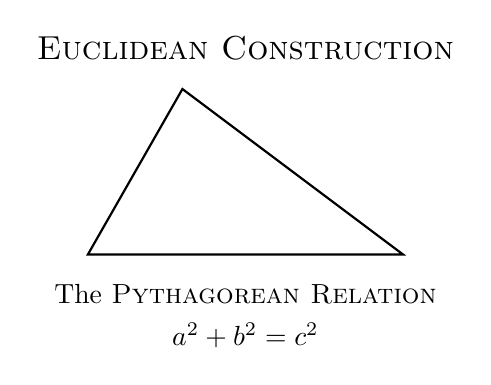
\begin{tikzpicture}
  \draw[thick] (0,0) -- (4,0) -- (1.2,2.1) -- cycle;
  \node[font=\large\scshape,anchor=south] at (2,2.35) {Euclidean Construction};
  \node[anchor=north] at (2,-0.25) {The \textsc{Pythagorean Relation}};
  \node[anchor=north] at (2,-0.75) {$a^2+b^2=c^2$};
\end{tikzpicture}
\end{document}
